\documentclass{article}\usepackage[]{graphicx}\usepackage[]{color}
%% maxwidth is the original width if it is less than linewidth
%% otherwise use linewidth (to make sure the graphics do not exceed the margin)
\makeatletter
\def\maxwidth{ %
  \ifdim\Gin@nat@width>\linewidth
    \linewidth
  \else
    \Gin@nat@width
  \fi
}
\makeatother

\definecolor{fgcolor}{rgb}{0.345, 0.345, 0.345}
\newcommand{\hlnum}[1]{\textcolor[rgb]{0.686,0.059,0.569}{#1}}%
\newcommand{\hlstr}[1]{\textcolor[rgb]{0.192,0.494,0.8}{#1}}%
\newcommand{\hlcom}[1]{\textcolor[rgb]{0.678,0.584,0.686}{\textit{#1}}}%
\newcommand{\hlopt}[1]{\textcolor[rgb]{0,0,0}{#1}}%
\newcommand{\hlstd}[1]{\textcolor[rgb]{0.345,0.345,0.345}{#1}}%
\newcommand{\hlkwa}[1]{\textcolor[rgb]{0.161,0.373,0.58}{\textbf{#1}}}%
\newcommand{\hlkwb}[1]{\textcolor[rgb]{0.69,0.353,0.396}{#1}}%
\newcommand{\hlkwc}[1]{\textcolor[rgb]{0.333,0.667,0.333}{#1}}%
\newcommand{\hlkwd}[1]{\textcolor[rgb]{0.737,0.353,0.396}{\textbf{#1}}}%

\usepackage{framed}
\makeatletter
\newenvironment{kframe}{%
 \def\at@end@of@kframe{}%
 \ifinner\ifhmode%
  \def\at@end@of@kframe{\end{minipage}}%
  \begin{minipage}{\columnwidth}%
 \fi\fi%
 \def\FrameCommand##1{\hskip\@totalleftmargin \hskip-\fboxsep
 \colorbox{shadecolor}{##1}\hskip-\fboxsep
     % There is no \\@totalrightmargin, so:
     \hskip-\linewidth \hskip-\@totalleftmargin \hskip\columnwidth}%
 \MakeFramed {\advance\hsize-\width
   \@totalleftmargin\z@ \linewidth\hsize
   \@setminipage}}%
 {\par\unskip\endMakeFramed%
 \at@end@of@kframe}
\makeatother

\definecolor{shadecolor}{rgb}{.97, .97, .97}
\definecolor{messagecolor}{rgb}{0, 0, 0}
\definecolor{warningcolor}{rgb}{1, 0, 1}
\definecolor{errorcolor}{rgb}{1, 0, 0}
\newenvironment{knitrout}{}{} % an empty environment to be redefined in TeX

\usepackage{alltt}
\usepackage{fullpage}
\title{STAT 675 HW \#6}
\author{Dominic LaRoche}
\IfFileExists{upquote.sty}{\usepackage{upquote}}{}
\begin{document}

\begin{itemize}
\item[11.1] The equality $log(exp(x))=exp(log(x))$ does not hold in computer computations because of insufficient precision.\\
\begin{knitrout}
\definecolor{shadecolor}{rgb}{0.969, 0.969, 0.969}\color{fgcolor}\begin{kframe}
\begin{alltt}
x = 10
\hlkwd{log}(\hlkwd{exp}(x)) == \hlkwd{exp}(\hlkwd{log}(x))
\end{alltt}
\begin{verbatim}
## [1] FALSE
\end{verbatim}
\begin{alltt}
\hlcom{# Using all.equal we can check if the identity holds with near equality}
\hlkwd{isTRUE}(\hlkwd{all.equal}(\hlkwd{log}(\hlkwd{exp}(x)), \hlkwd{exp}(\hlkwd{log}(x))))
\end{alltt}
\begin{verbatim}
## [1] TRUE
\end{verbatim}
\begin{alltt}

\hlcom{# interestingly R can habdle the case where x=0 or 1 setting both sides to}
\hlcom{# precisely 1 or 0 respectively}
x = 1
\hlkwd{log}(\hlkwd{exp}(x)) == \hlkwd{exp}(\hlkwd{log}(x))
\end{alltt}
\begin{verbatim}
## [1] TRUE
\end{verbatim}
\begin{alltt}
x = 0
\hlkwd{log}(\hlkwd{exp}(x)) == \hlkwd{exp}(\hlkwd{log}(x))
\end{alltt}
\begin{verbatim}
## [1] TRUE
\end{verbatim}
\end{kframe}
\end{knitrout}


\item[11.4] Intersection points of two curves in a bounded region (o,$sqrt{k}$).\\
\begin{knitrout}
\definecolor{shadecolor}{rgb}{0.969, 0.969, 0.969}\color{fgcolor}\begin{kframe}
\begin{alltt}
K <- \hlkwd{c}(4:25, 100, 500, 1000)
eq <- \hlkwd{function}(a, k) \{
\hlcom{    # since we are looking for p(t>x) we can use pt with the option}
\hlcom{    # lower.tail=FALSE}
    sk1 <- \hlkwd{pt}(\hlkwd{sqrt}((a^2 * (k - 1))/(k - a^2)), df = k - 1, lower.tail = F)
    sk <- \hlkwd{pt}(\hlkwd{sqrt}(((a^2) * k)/(k + 1 - a^2)), df = k, lower.tail = F)
    \hlkwd{return}(sk1 - sk)
\}
\hlkwd{par}(mfrow = \hlkwd{c}(2, 2))
\hlkwd{curve}(\hlkwd{eq}(a = x, k = 4), xlim = \hlkwd{c}(0, 2))
\hlkwd{abline}(a = 0, b = 0)
\hlkwd{curve}(\hlkwd{eq}(a = x, k = 25), xlim = \hlkwd{c}(0, 5))
\hlkwd{abline}(a = 0, b = 0)
\hlkwd{curve}(\hlkwd{eq}(a = x, k = 500), xlim = \hlkwd{c}(0, \hlkwd{sqrt}(500)))
\end{alltt}


{\ttfamily\noindent\color{warningcolor}{\#\# Warning: NaNs produced}}\begin{alltt}
\hlkwd{abline}(a = 0, b = 0)
\hlkwd{par}(mfrow = \hlkwd{c}(1, 1))
\end{alltt}
\end{kframe}
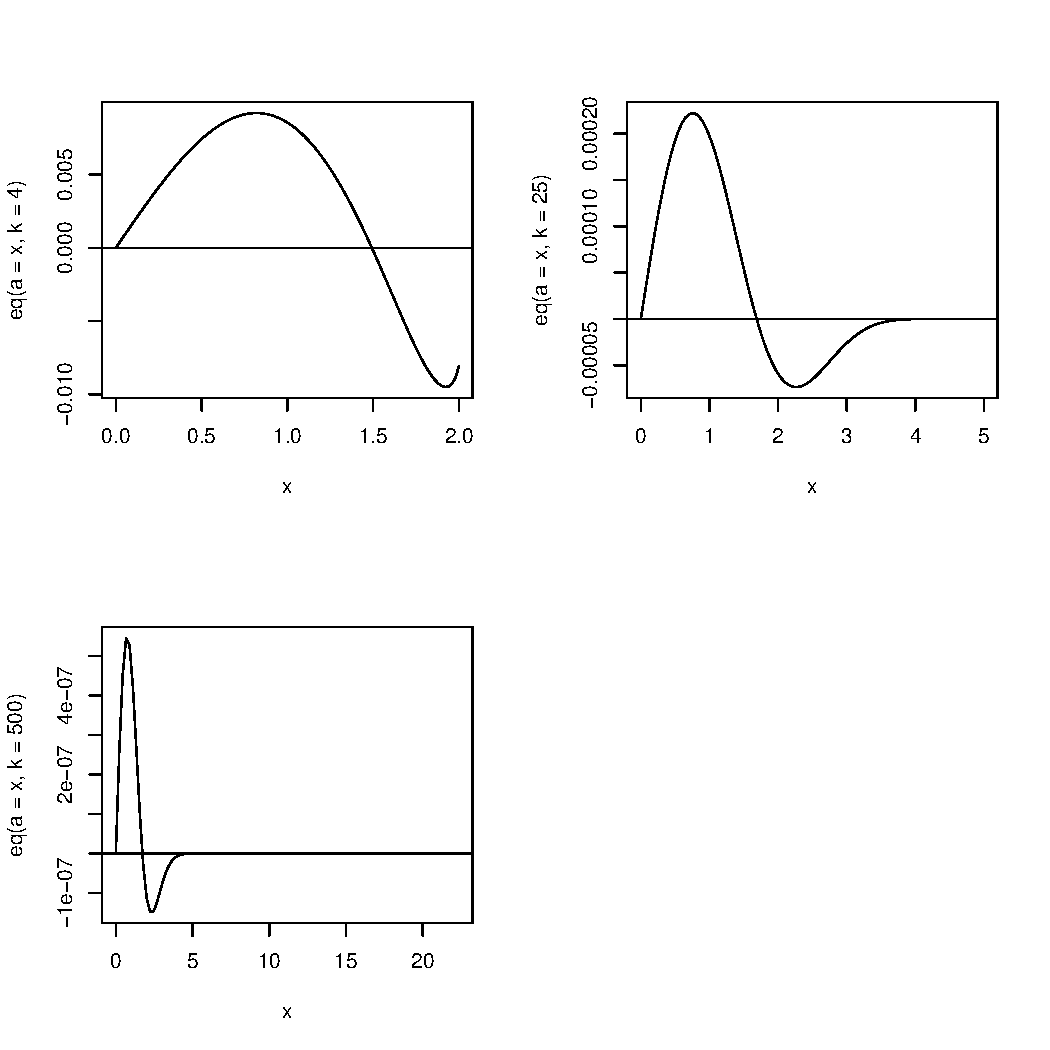
\includegraphics[width=\maxwidth]{figure/eleven4} 
\begin{kframe}\begin{alltt}
\hlcom{# it appears we can bound the search by 0.1 and 2 instead of 0 and sqrt(k)}
roots <- \hlkwd{numeric}(\hlkwd{length}(K))
\hlkwd{for} (i in 1:\hlkwd{length}(K)) \{
    roots[i] <- \hlkwd{uniroot}(f = eq, interval = \hlkwd{c}(0.1, 2), k = K[i])$root
\}
\hlkwd{cbind}(k, roots)
\end{alltt}


{\ttfamily\noindent\bfseries\color{errorcolor}{\#\# Error: object 'k' not found}}\end{kframe}
\end{knitrout}


\item[11.6]  Cauchy CDF.\\
\begin{knitrout}
\definecolor{shadecolor}{rgb}{0.969, 0.969, 0.969}\color{fgcolor}\begin{kframe}
\begin{alltt}
cauch.pdf <- \hlkwd{function}(x, eta, theta) \{
    \hlkwd{return}(1/(theta * pi * (1 + ((x - eta)/theta)^2)))
\}
p.cauch <- \hlkwd{function}(q, theta, eta, lower.tail = TRUE) \{
    \hlkwd{return}(\hlkwd{integrate}(f = cauch.pdf, lower = -Inf, upper = q, theta = theta, 
        eta = eta)$value)
\}
quants <- \hlkwd{matrix}(1:5, 5, 1)
mine <- \hlkwd{apply}(quants, 1, p.cauch, theta = 1, eta = 0)
bases <- \hlkwd{pcauchy}(quants)
\hlkwd{cbind}(quants, mine, bases)
\end{alltt}
\begin{verbatim}
##          mine       
## [1,] 1 0.7500 0.7500
## [2,] 2 0.8524 0.8524
## [3,] 3 0.8976 0.8976
## [4,] 4 0.9220 0.9220
## [5,] 5 0.9372 0.9372
\end{verbatim}
\begin{alltt}
\hlkwd{for} (i in 1:5) \{
    \hlkwd{print}(\hlkwd{isTRUE}(\hlkwd{all.equal}(mine[i], bases[i])))
\}
\end{alltt}
\begin{verbatim}
## [1] TRUE
## [1] TRUE
## [1] TRUE
## [1] TRUE
## [1] TRUE
\end{verbatim}
\begin{alltt}
\hlcom{# the quantiles compare very favorably when using the standard cauchy}
mine <- \hlkwd{apply}(quants, 1, p.cauch, theta = 2, eta = 2)
bases <- \hlkwd{pcauchy}(quants, location = 2, scale = 2)
\hlkwd{cbind}(quants, mine, bases)
\end{alltt}
\begin{verbatim}
##          mine       
## [1,] 1 0.3524 0.3524
## [2,] 2 0.5000 0.5000
## [3,] 3 0.6476 0.6476
## [4,] 4 0.7500 0.7500
## [5,] 5 0.8128 0.8128
\end{verbatim}
\begin{alltt}
\hlkwd{for} (i in 1:5) \{
    \hlkwd{print}(\hlkwd{isTRUE}(\hlkwd{all.equal}(mine[i], bases[i])))
\}
\end{alltt}
\begin{verbatim}
## [1] TRUE
## [1] TRUE
## [1] TRUE
## [1] TRUE
## [1] TRUE
\end{verbatim}
\begin{alltt}
\hlcom{# changing the scale and location parameters does not affect the precision}
\hlcom{# outside of computer tolerance}
\end{alltt}
\end{kframe}
\end{knitrout}

\item[11.7]  Application of the simplex method.\\
\begin{knitrout}
\definecolor{shadecolor}{rgb}{0.969, 0.969, 0.969}\color{fgcolor}\begin{kframe}
\begin{alltt}
\hlkwd{library}(boot)
A1 <- \hlkwd{rbind}(\hlkwd{c}(2, 1, 1), \hlkwd{c}(1, -1, 3))
b1 <- \hlkwd{c}(2, 3)
a <- \hlkwd{c}(4, 2, 9)
\hlkwd{simplex}(a = a, A1 = A1, b1 = b1, maxi = TRUE)
\end{alltt}
\begin{verbatim}
## 
## Linear Programming Results
## 
## Call : simplex(a = a, A1 = A1, b1 = b1, maxi = TRUE)
## 
## Maximization Problem with Objective Function Coefficients
## x1 x2 x3 
##  4  2  9 
## 
## 
## Optimal solution has the following values
##   x1   x2   x3 
## 0.00 0.75 1.25 
## The optimal value of the objective  function is 12.75.
\end{verbatim}
\end{kframe}
\end{knitrout}


\item[11.A] The complete log likelihood is:\\
$$f_{x,x_{n+1}}(X,X_{n+1}|\theta)=f_{x_{n+1}|x}(X_{n+1}|X,\theta) f_x(X|\theta)$$
where $X=\sum_{i=1}^n x_i \sim Gamma(n,\theta)$ since $x_1 ... x_n$ iid Exp($\theta$).  Using the independence of $X$ and $X_{n+1}$ the full likelihood then becomes,\\
$l(\theta|X_{i...n},X_{n+1})=log\left[\frac{\theta^n X^{n-1} e^{-\theta X}}{\Gamma(n)}\right]+log\theta - \theta X_{n+1}$\\

$=nlog\theta + (n-1)logX -\theta X - log \Gamma(n) + log\theta - \theta X_{n+1}$\\

$=(n+1)log\theta + (n-1)logX - log\Gamma(n) - \theta(X+X_{n+1})$\\

\textbf{The E-step is then:}
$Q(\theta,\theta_{t-1})=E[l(\theta|X_{i...n},X_{n+1})|X,\theta_{t-1}]$\\

$=E[(n+1)log\theta + (n-1)logX - log\Gamma(n) - \theta(X+X_{n+1})|X,\theta_{t-1}]$\\

$=(n+1)log\theta + (n-1)logX - log\Gamma(n) - \theta(X + E(X_{n+1}|\theta_{t-1}))$\\

$=(n+1)log\theta + (n-1)logX - log\Gamma(n) - \theta\left(X + \frac{1}{\theta_{t-1}}\right)$\\

\textbf{The M-step is then to maximize Q}:\\
$\frac{dQ}{d\theta} - x + \frac{1}{\theta_{t-1}}$, set equal to 0 and solve for $\theta$.\\

$\theta_t = \frac{(n+1)\theta_{t-1}}{x \theta_{t-1}+1}$


\begin{knitrout}
\definecolor{shadecolor}{rgb}{0.969, 0.969, 0.969}\color{fgcolor}\begin{kframe}
\begin{alltt}
tol = \hlkwd{sqrt}(.Machine$double.eps)

update = \hlkwd{function}(theta, x1, n) \{
    ((n + 1) * theta)/(1 + x1 * theta)
\}
Q = \hlkwd{function}(th, th1, x1, n) \{
    (n + 1) * \hlkwd{log}(th) + (n - 1) * \hlkwd{log}(x1) - \hlkwd{lgamma}(n) - th * (x1 + (1/th1))
\}

x <- \hlkwd{c}(840, 157, 145, 44, 33, 121, 150, 280, 434, 736, 584, 887, 263, 1901, 
    695, 294, 562, 721, 76, 710, 46, 402, 194, 759, 319, 460, 40, 1336, 335, 
    1354, 454, 36, 667, 40, 556, 99, 304, 375, 567, 139, 780, 203, 436, 30, 
    384, 1299, 9, 209, 599, 83, 832, 328, 126, 1617, 638, 937, 735, 38, 365, 
    92, 82, 220)
x1 = \hlkwd{sum}(x)  \hlcom{# observed datum}
n = 62
theta = 1  \hlcom{#theta0 initial guess}
thetaold = theta

\hlkwd{while} (\hlkwd{abs}(\hlkwd{Q}(\hlkwd{update}(theta, x1, n), theta, x1, n) - \hlkwd{Q}(theta, thetaold, x1, n)) > 
    tol) \{
    thetaold = theta
    theta = \hlkwd{update}(theta, x1, n)
    \hlkwd{print}(theta)
\}
\end{alltt}
\begin{verbatim}
## [1] 0.002237
## [1] 0.002202
## [1] 0.002202
## [1] 0.002202
## [1] 0.002202
## [1] 0.002202
\end{verbatim}
\end{kframe}
\end{knitrout}

\end{itemize}
\end{document}
